\documentclass{pete-wcp}
\paperwidth=8.5in
\paperheight=11in

\newfont{\mycrnotice}{ptmr8t at 7pt}
\newfont{\myconfname}{ptmri8t at 7pt}
\let\crnotice\mycrnotice%
\let\confname\myconfname%

\clubpenalty=10000
\widowpenalty=10000

% \usepackage{epsfig}
% \usepackage{fancyvrb}
% \usepackage{graphicx}
% \usepackage{subfigure}
% \usepackage{pifont}
\usepackage{algorithm}
\usepackage{algorithmic}
\usepackage{booktabs}
\usepackage[hyphens]{url}
% \usepackage{xspace}
\usepackage[numbers]{natbib}
\usepackage{verbatim}
\usepackage{microtype}
\usepackage{framed}
\usepackage[lofdepth,lotdepth]{subfig}
% \usepackage{comment}

% All information about acronyms and abbreviations are handled in
% a single file for possible reuse
\usepackage{acronym}

\acrodef{SFE}[SFE]{Secure function evaluation}
\acrodef{OT}[OT]{oblivious transfer}
\acrodef{GCP}[GCP]{\emph{garbled circuits protocol}}
\acrodef{P1}[\emph{P1}]{the first party}
\acrodef{P2}[\emph{P2}]{the second party}
\acrodef{f}[\emph{f}]{a function to execute}

\newcommand{\ponein}{$i_{P1}$}
\newcommand{\ptwoin}{$i_{P2}$}




\renewcommand*{\bibfont}{\raggedright}


\begin{document}

\title{Yao's Garbled Circuits:\\Recent Directions and Implementations}
\numberofauthors{1}
\author{
    \alignauthor
        Peter Snyder \\
           \affaddr{University of Illinois at Chicago}\\
           \affaddr{Chicago, Illinois, USA}
           \email{psndye2@uic.edu}
}

\date{25 March 2014}

\maketitle
\begin{abstract}
    Secure function evaluation, or how two parties can jointly compute a function without any other party learning about any other party's inputs, has been an active field in cryptography. In 1986 Andrew Yao presented a solution to the problem called \emph{garbled circuits}, based on modeling the problem as a series of binary gates and encrypting the result tables. This approach was initial treated as theoretically interesting but too computationally expensive for practical use.  However, in the decades since Yao's solution was initially published, much work has gone into both optimizing the protocol for practical use, and further securing the protocol to make it further secure.

This paper provides a thorough explanation of both Yao's original protocol and its security characteristics.  The paper then details additions to the protocol to make it both practical for computation and secure against untrusted parties.  Implementations of Yao's protocol are also discussed, though the paper's emphasis is on the underlying enabling improvements to the protocol.

\end{abstract}

\section{Introduction}
\label{sec:intro}

\ac{SFE} referrers to the problem of how can two parties collaborate to correctly compute the output of a function without any party needing to reveal their inputs to the function, either to each other or to a third party.  A common example of this problem is the ``millionaires problem'', in which two millionaires wish to determine which of them has more money, without either party revealing how much money they have\cite{yao1982protocols}.

Many solutions have been developed for \ac{SFE}. One category of solution is function specific, and depends on specific attributes of the function being executed to provide security\cite{huang2011faster}.  These solutions, while interesting, are by definition of less general interest, since they apply to only a limited set of problems.

Another category of approach is more general, and seeks to provide a general solution for \ac{SFE} by transforming arbitrary functions into secure functions. Approaches in this category include homomorphic encryption systems\cite{gentry2009fully} which allow for arbitrary execution on encrypted data.  Yao's \emph{garbled circuits} protocol fits in this second category.

Yao's \ac{GCP} transforms any function into a function that can be evaluated securely by modeling the function as a boolean circuit, and then masking the inputs and outputs of each gate so that the party executing the function cannot discern any information about the inputs or intermediate values of the function. The protocol is secure as long as both parties follow the protocol. A full description of the protocol and the related security definitions are provided later in this paper.

\subsection{History of Protocol}

Interestingly, Yao never published his \ac{GCP}. Several of his publications discuss approaches to the \ac{SFE} problem generally, specifically papers from 1982\cite{yao1982protocols} and 1986\cite{yao1986generate}. These papers are much broader in scope and are much more abstract than providing a protocol that could be implemented. Yao first discussed the \emph{garbled circuits} approach in a public talk on the latter paper, as a concrete example of how his broader strategies could be applied\cite{bellare2012foundations}. Only later and by other researchers would the protocol be documented formally\cite{goldreich1987play}, though still crediting Yao for the approach.

Yao having developed this foundational protocol, but never having published it, presents authors with the tricky question of what to cite when crediting to the \ac{GCP} approach.  The common approach seems to be to cite Yao's two papers discussing his general approach the problem, even though those papers make no mention of garbled circuits or any similar concept.

\subsection{Aims of the Paper}

This paper aims to provide a full description of Yao's \ac{GCP} and its security characteristics, namely what security the protocol does and does not provide.  This paper also provides detailed explanations of related work done by other authors to improve the performance and security provided by the protocol.

This paper presumes no previous familiarity with Yao's protocol or cryptography in general in the explanation explanation of the protocol, beyond the general concepts of symmetric and asymmetric cryptography.  Some background in cryptography is assumed in the sections on improvements and additions to the protocol.  Formal proofs of the underlying concepts are not discussed and are left to their originating papers.

Some discussion is included of existing implementations of Yao's protocol. However, the focus here is on the promises, improvements and general techniques of the implementations, and not on implementation details like programming languages or hardware characteristics. Discussion of the implementations is mainly meant to inform how the protocol has developed and been improved, as opposed to a detailed comparison of how different implementations compare with each other.
\pagebreak
\subsection{Organization of the Paper}

The remainder of the paper is structured as follows. Section \ref{sec:definitions} provides some security definitions used throughout the rest of the paper. Section \ref{sec:ot} discusses \ac{OT}, its role in the protocol, and a method for achieving \ac{OT} in a manner that is compatible with the security guarantees of the standard version of Yao's protocol.  Section \ref{sec:protocol} then provides a full explanation of the Yao's protocol and how to use \emph{garbled circuits} to solve the \emph{SFE} problem. Section \ref{sec:security} discusses the security of the protocol and proposed improvements, and \ref{sec:performance} provides a similar discussion of performance issues in Yao's protocol. Section \ref{sec:implementations} provides a brief overview of some implementations of the protocol, and section \ref{sec:conclusion} concludes.

\section{Security Definitions}
\label{sec:definitions}

This section defines several security related terms that are used through out this paper.  The terminology is not identical throughout the literature, but have mappings onto similar, equivalent terms.


\subsection{Properties of \ac{SFE} System}

Attempting to abstractly but precisely defining the characteristics of a \ac{SFE} protocol is difficult and can quickly devolve into a long enumeration of characteristics a \ac{SFE} system should \emph{not} do.  Instead, Yao suggests\cite{yao1986generate} that a correct system should be compared to an ideal-oracle that fulfills three properties, and that a \ac{SFE} system is correct if it performs identically to this imagined ideal-oracle.

This imagined ideal-oracle takes \ac{f}, \ac{P1}'s input (\ponein) and \ac{P2}'s input (\ptwoin), executes the given function with the values provided, and then returns the function's output to both parties ($u \leftarrow f(i_{P1}, i_{P2})$).


\subsubsection{Validity}

A \ac{SFE} system must perform indistinguishably from an ideal-oracle in being able to correctly calculate the given function. Note that this does not guarantee a correct result, since the function being computed in a secure manner could itself have a logic error in it, nor does it guarantee to produce any answer, if one of the parties submits an invalid input to the computation. This \emph{validity} requirement merely requires that the function produce the same result as the insecure (or ``pre-secured'') version of the function being evaluated, given the same inputs.


\subsubsection{Privacy}

A \ac{SFE} system must also perform indistinguishably from an ideal-oracle in preventing preventing \ac{P2} from learning about \ponein\, provided \ac{P1} follows the protocol.  The same must also hold for preventing \ac{P1} from learning about \ptwoin.

Note that that this definition of \emph{privacy} does not guarantee that \ac{P1} is not able to learn \ac{P2}'s input by examining the function's result (if the function being executed allows for such reverse engineering).  If, for example, the function being evaluated securely is multiplication, the fact that \ac{P1} can learn \ptwoin\ through $u/i_{P1}$ does not violate this \emph{privacy} property; \ac{P1} could learn \ptwoin\ in this scenario given an ideal-oracle as well.

This does not imply that \ac{SFE} cannot be used to protect the \emph{privacy} of each parties' inputs, only that some functions (such as integer multiplication) do not make sense in the context of \ac{SFE}.

\subsubsection{Fairness}

Finally, a \ac{SFE} system must perform indistinguishably from an ideal-oracle in preventing one party from learning the output of \emph{f} while learning it themselves.  In order words, \ac{P1} should not be able to learn the output of \emph{f} while denying it to \ac{P2}, and vise-versa.

\subsection{Adversary Models}

In addition to defining the properties a \ac{SFE} should have, its necessary to define under which conditions those properties must hold.  While the relevant literature contains many different terms for an adversary's willingness to deviate from the protocol, and many gradations between 100\% honest and 100\% malicious, this paper generalizes the types of attackers into two categories, at the extremes of the attacker spectrum.

A \ac{SFE} protocol is said to be secure against under a given adversary model if the given \ac{SFE} protocol can provide the three above mentioned security properties against any party following the assumptions of the adversary model.

\subsubsection{Semi-Honest}

A \emph{semi-honest} adversary is assumed to follow all required steps in a protocol, but will also look for all advantageous information leaked from the execution of the protocol, such as intermediate values, control flow decisions, or values derivable from the same\cite{goldreich1998secure}.  Additionally, \emph{semi-honest} adversaries are assumed to be selfish, in that they will take any steps that will benefit themselves if the benefit is greater than the harm, within the constraints imposed by the protocol.


\subsubsection{Malicious}

A \emph{malicious} adversary is assumed to arbitrarily deviate from the protocol at any point, and in whenever way it might benefit them\cite{goldreich1998secure}.  This includes proving deceptive or incorrect values, aborting a protocol at anytime, or otherwise taking any steps that could reach a desirable outcome.  This is the most difficult type of adversary to secure against; a system that is secure against \emph{malicious} adversaries is also therefor secure against \emph{semi-honest} adversaries.


\subsection{Hash Functions}

This paper is written with the assumption that has functions, or at least some efficient hash function, models a random oracle, or that the hash function can be treated as a random mapping from $f(\{0, 1\}^{*}) \to \{0, 1\}^{h}$, where $h$ is the length of the produced message digest.  This assumption implies that there is no correlation between the output of a hash function and its input.  Or, put differently, that nothing can be learned about the input to a hash function by examining its output.

This assumption is a common one throughout the field and discussed research\cite{pinkas2009secure}.  Where work mentions alternate constructions or other caveats if this random oracle assumption does not hold, they are mentioned.

\section{Oblivious Transfer}

\ac{OT} refers to methods for two parties to exchange 1 of several values, with the sending party blinded to what value was selected, and the receiving party blinding to all other possible values that could have, but were not selected.

While \ac{OT} and \ac{SFE} are approaches to distinct (though related) problems, understanding the Yao's \ac{GCP} and the security properties requires some understanding of \ac{OT} and how it is used in the protocol. Its a cryptographic primitive that serves as a building block that the security of Yao's \ac{GCP} relies on.

This section provides a brief overview of the \ac{OT} problem, a simple protocol that provides a solution to the \ac{OT} problem against \emph{semi-honest} adversaries. The role of \ac{OT} in Yao's protocol is discussed in section 4.

\subsection{Problem Definition}

A general form of \ac{OT} is \emph{1-out-of-N oblivious transfer}, a two party protocol where \ac{P1}, the sending party, has a collection of values. \ac{P2} is able to select one of the values from this set to receive, but is not able to learn any of the other values.

More formally, a \emph{1-out-of-N oblivious transfer} protocol takes as inputs a set of values \emph{N} from \ac{P1}, and \emph{i} form \ac{P2}, where
$0 \leq i < |N|$. The protocol then outputs nothing to \ac{P1}, and $N_i$ to \ac{P2} in a manner that prevents \ac{P2} from learning another other values in \emph{N}.

A special case of the above is the \emph{1-out-of-2 oblivious transfer} problem, where \emph{N} is fixed at 2.  Here \ac{P1} has just two values, and \ac{P2} is accordingly limited to $i \in \{0, 1\}$.  All versions of Yao's \ac{GCP} discussed in this paper rely on \emph{1-out-of-2 oblivious transfer} protocols.

\subsection{Example 1-out-of-2 Protocol}

The problem of \emph{1-out-of-2 \ac{OT}} was first addressed by Rabin\cite{rabin2005exchange} in 1981 using an online approach with multiple rounds of message passing, but was later adapted into an offline approaches using an techniques similar to the Diffie-Hellman key exchange protocol\cite{diffie1976new}.

The following protocol\cite{lindell2013technion} is a very simple \emph{1-out-of-2 \ac{OT}} protocol that is secure against \emph{semi-honest}. It is included here to help in the next section's explanation of how the full \ac{GCP} works, and to provide a easy-to-understand example of \ac{OT} to build from later.

\begin{algorithm}[H]
    \floatname{algorithm}{Protocol}
    \caption{Semi-Honest 1-out-of-2 Oblivious Transfer}
    \label{alg:otsemihonest}
    \begin{algorithmic}[1]
        \STATE \ac{P1} has a set of two strings, $S = \{s_0, s_1\}$.
        \STATE \ac{P2} selects $i \in \{0, 1\}$ corresponding to whether she wishes to learn the $s_0$ or $s_1$.
        \STATE \ac{P2} generates two pairs of public / private keys,\\
        $(k^{pub}_0, k^{pri}_0), (k^{pub}_1, k^{pri}_1)$.
        \STATE \ac{P2} then destroys $k^{pri}_{i-1}$, preventing her from recovering any information encrypted under $k^{pub}_{i-1}$.
        \STATE \ac{P1} generates $c_0 = E_{k^{pub}_0}(s_0)$ and $c_1 = E_{k^{pub}_1}(s_1)$ and sends $c_0$ and $c_1$ to \ac{P2}.
        \STATE \ac{P2} computes $s_i = D_{k^{pri}_i}(c_i)$.
    \end{algorithmic}
\end{algorithm}

Note that that as long as all parties follow the protocol, the protocol is secure by the \emph{semi-honest} definition. \ac{P2} is able to recover the desired string from \emph{S} but is not able to recover the other value from \emph{S}. Similarly, \ac{P1} does not know which value from \emph{S} \ac{P2} learned.

\section{Yao's Protocol}
\label{sec:protocol}

This section provides a complete description of Yao's \emph{garbled circuits protocol} and how the protocol incorporates \ac{OT}.  Though the protocol described here was first published by Goldreich, Micali, and Wigderson\cite{goldreich1987play}, the terminology used in this section follows more recent publications\cite{hazay2010efficient}. In all cases though the concepts are similar and there is a direct mapping between the two.

The protocol is presented here twice, first in a less formal format that includes some reasoning for each step in the protocol, and a second time, fully describing each step taken by both parties. The former description is intended to make the latter one easier to follow.

\begin{algorithm}[H]
    \floatname{algorithm}{Protocol}
    \caption{Yao's Garbled Circuits Protocol}
    \label{alg:yao}
    \begin{algorithmic}[1]
        \STATE \ac{P1} generates a boolean circuit representation $c_c$ of \ac{f} that takes input $i_{P1}$ from \ac{P1} and $i_{P2}$ from \ac{P2}.
        \STATE \ac{P1} transforms $c_c$ by garbling each gate's computation table, creating garbled circuit $c_g$.
        \STATE \ac{P1} sends both $c_g$ and the values for the input wires in $c_g$ corresponding to $i_{P1}$ to \ac{P2}.
        \STATE \ac{P2} uses \emph{1-out-of-2 \ac{OT}} to receive from \ac{P1} the garbled values for $i_{P2}$ in $c_g$.
        \STATE \ac{P2} calculates $c_g$ with the garbled versions of $i_{P1}$ and $i_{P2}$ and outputs the result.
    \end{algorithmic}
\end{algorithm}

\subsection{Intuitive Description of the Protocol}

This section attempts to provide a high level explanation of how Yao's protocol works, as well as some of the reasoning behind its construction. It is included to make the following detailed description of the protocol easier to follow.

\ac{P1} and \ac{P2} wish to compute function \emph{f} securely, so that their inputs to the function remain secret. They begin doing so by modeling \emph{f} as a boolean circuit. \ac{P1} then ``garbles'' the circuit by replacing all boolean values in the circuit with pseudo-random looking strings, and then keeping this mapping secret.  This is done for the input and output wires of every gate in the circuit, with the exception of the circuits output gates; the values of these gates' output wires are left un-garbled.

\ac{P1} then replaces each bit of his input with the pseudo-random string that maps to that bit's input on the corresponding input wire into circuit. \ac{P1} then sends the garbled circuit and his garbled input to \ac{P2}.

\ac{P2} receives both the garbled circuit and \ac{P1}'s garbled input. However, since all input wires into the circuit have been garbled and only \ac{P1} has the mapping between the garbled values and the underlying bits, \ac{P2} does not know what values to input into the circuit to match her input bits. In other words, for each input wire into the circuit, \ac{P2} can select one of two random strings to input (corresponding to 0 or 1), but does not know which of these correspond to her desired input bit.

In order to learn which pseudo-random string to select for each of \ac{P2}'s input wires, \ac{P2} engages in a \emph{1-out-of-2 \ac{OT}} with \ac{P1} for each bit of \ac{P2}'s input. For each round of the \ac{OT}, \ac{P2} submits the bit she wishes to learn, receives the corresponding string.  Note that the properties of \ac{OT} prevent \ac{P1} from learning about \ac{P2}'s input in this process.

Once \ac{P2} has received all of the strings corresponding to her input into the circuit, she holds everything needed to compute the output of the circuit: her garbled inputs, \ac{P1}'s garbled inputs, and the garbled circuit itself. Further, she has obtained these values without \ac{P1} learning her inputs, nor \ac{P2} learning \ac{P1}'s inputs.

\ac{P2} then begins to compute the circuit by entering the pseudo-random strings that correspond to each bit of her and \ac{P1}'s input into the corresponding input wire and using the resulting garbled output string as an input to the next gate. \ac{P2} may try to learn information about \ac{P1}'s inputs by watching the execution of the circuit. The protocol prevents \ac{P2} from doing so though the manner that each computation table for each gate was constructed.

Recall that the computation table for every gate in the circuit was constructed so that each pair of inputs produces a output string that represents the correct boolean result, but which appears pseudo-random to \ac{P2}.  In other words, instead of mapping from $\{0, 1\} \times \{0, 1\} \to \{0, 1\}$, all gates in the circuit become a function mapping two random looking strings to another uniformly distributed pseudo-random string, or $f(\{0, 1\}^{|k|}, \{0, 1\}^{|k|}) \to \{0, 1\}^{|k|}$, where $|k|$ is the size of the value returned by the hash function. Since \ac{P2} never learns the mapping between strings used in the table and their underlying boolean values, \ac{P2} learns nothing by watching the outputs of each gate.

Recall that the values returned by the output gates in the circuit are not obscured. This results in \ac{P2} learning the value of $f(i_{P1}, i_{P2})$ once the computation has finished.  \ac{P2} then completes the protocol by sharing this computed value with \ac{P1}.


\subsection{Detailed Description of the Protocol}

This section provides a more precise explanation of each step of Yao's protocol, specifying how each step of the is carried out by both parties.  The numbering of subsections here followings the numbering used in protocol \ref{alg:yao}.


\subsubsection{Generating A Boolean Circuit Representation of the Function}

Before it can be securely evaluated, the function \emph{f} must be converted into an equivalent boolean circuit $c$ so that $\forall x, y \rightarrow f(x, y) = c(x, y)$. The strategies for optimally doing so may be function specific, and are beyond the scope of the protocol.  For the purposes of this paper though, it is sufficient to note that there exists a mapping from any polynomial time function with fixed sized inputs to a boolean circuit that calculates the same output\cite{goldreich1987play}.


\subsubsection{Garbling Truth Tables}

Once \ac{P1} has constructed a boolean circuit representation $c$ of $f$, the next step is to garble the truth table for each gate in $c$, generating a garbled version of the circuit, $c_g$ (ie $c \to c_g$).

\begin{figure}[t]
    \centering
    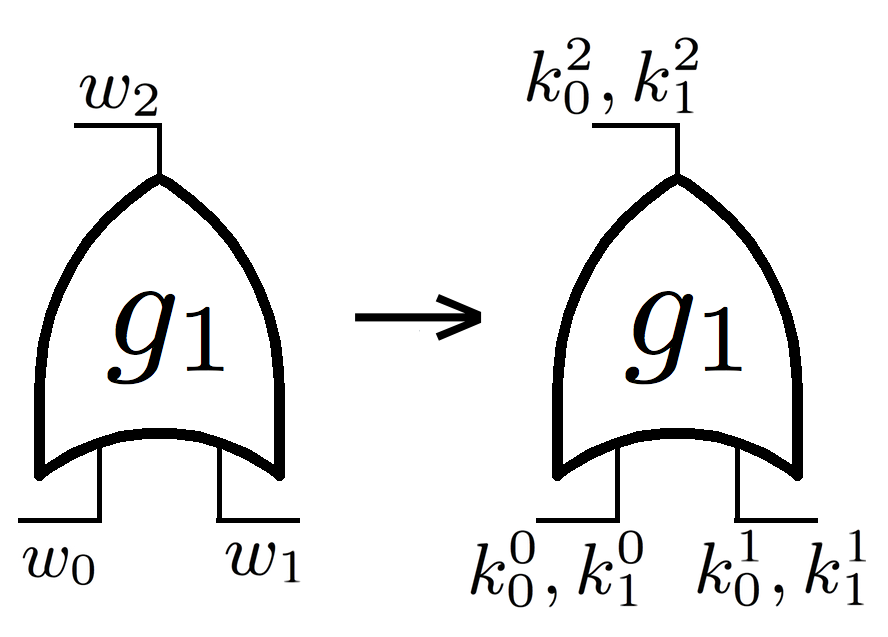
\includegraphics[width=\columnwidth]{images/or_gate}
    \caption{Garbling a single gate}
    \label{fig:garblegateimg}

    \subfloat[Original Values]{
        \begin{tabular}{ c | c || c }
            \hline
            $w_0$ & $w_1$ & $w_2$ \\
            \hline
            0 & 0 & 0 \\
            \hline
            0 & 1 & 1 \\
            \hline
            1 & 0 & 1 \\
            \hline
            1 & 1 & 1 \\
            \hline
        \end{tabular}
        \label{fig:gategarblepre}
    }
    \subfloat[Garbled Values]{
        \begin{tabular}{ c | c || c || c }
            \hline
            $w_0$ & $w_1$ & $w_2$ & garbled value \\
            \hline
            $k^0_0$ & $k^0_1$ & $k^0_2$ & $H(k^0_0 || k^0_1 || g_1) \oplus k^0_2$\\
            \hline
            $k^0_0$ & $k^1_1$ & $k^1_2$ & $H(k^0_0 || k^1_1 || g_1) \oplus k^1_2$\\
            \hline
            $k^1_0$ & $k^0_1$ & $k^1_2$ & $H(k^1_0 || k^0_1 || g_1) \oplus k^1_2$\\
            \hline
            $k^1_0$ & $k^1_1$ & $k^1_2$ & $H(k^1_0 || k^1_1 || g_1) \oplus k^1_2$\\
            \hline
        \end{tabular}
        \label{fig:gategarblepost}
    }
    \caption{Computation table for $g^{OR}_1$}
    \label{fig:gategarble}
\end{figure}

\begin{figure}[t!]
    \centering
    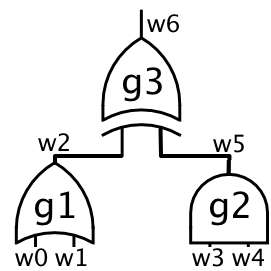
\includegraphics[width=\columnwidth]{images/multi_gates}
    \caption{Composing several gates into a simple circuit}
    \label{fig:garblecircuitimg}
    \subfloat[Original Values]{
        \begin{tabular}{ c | c || c }
            \hline
            $w_3$ & $w_4$ & $w_5$ \\
            \hline
            0 & 0 & 0 \\
            \hline
            0 & 1 & 0 \\
            \hline
            1 & 0 & 0 \\
            \hline
            1 & 1 & 1 \\
            \hline
        \end{tabular}
        \label{fig:andgatepre}
    }
    \subfloat[Garbled Values]{
        \begin{tabular}{ c | c || c || c }
            \hline
            $w_3$ & $w_4$ & $w_5$ & garbled value \\
            \hline
            $k^0_3$ & $k^0_4$ & $k^0_5$ & $H(k^0_3 || k^0_4 || g_2) \oplus k^0_5$\\
            \hline
            $k^0_3$ & $k^1_4$ & $k^0_5$ & $H(k^0_3 || k^1_4 || g_2) \oplus k^0_5$\\
            \hline
            $k^1_3$ & $k^0_4$ & $k^0_5$ & $H(k^1_3 || k^0_4 || g_2) \oplus k^0_5$\\
            \hline
            $k^1_3$ & $k^1_4$ & $k^1_5$ & $H(k^1_3 || k^1_4 || g_2) \oplus k^1_5$\\
            \hline
        \end{tabular}
        \label{fig:andgatepost}
    }
    \caption{Computation table for $g^{AND}_2$}
    \label{fig:andgate}

    \subfloat[Original Values]{
        \begin{tabular}{ c | c || c }
            \hline
            $w_2$ & $w_5$ & $w_6$ \\
            \hline
            0 & 0 & 0 \\
            \hline
            0 & 1 & 1 \\
            \hline
            1 & 0 & 1 \\
            \hline
            1 & 1 & 0 \\
            \hline
        \end{tabular}
        \label{fig:xorgatepre}
    }
    \subfloat[Garbled Values]{
        \begin{tabular}{ c | c || c || c }
            \hline
            $w_2$ & $w_5$ & $w_6$ & garbled value \\
            \hline
            $k^0_2$ & $k^0_5$ & $k^0_6$ & $H(k^0_2 || k^0_5 || g_3) \oplus k^0_6$\\
            \hline
            $k^0_2$ & $k^1_5$ & $k^1_6$ & $H(k^0_2 || k^1_5 || g_3) \oplus k^1_6$\\
            \hline
            $k^1_2$ & $k^0_5$ & $k^1_6$ & $H(k^1_2 || k^0_5 || g_3) \oplus k^1_6$\\
            \hline
            $k^1_2$ & $k^1_5$ & $k^0_6$ & $H(k^1_2 || k^1_5 || g_3) \oplus k^0_6$\\
            \hline
        \end{tabular}
        \label{fig:xorgatepost}
    }
    \caption{Computation table for $g^{XOR}_3$}
    \label{fig:xorgate}
\end{figure}

To see how \ac{P1} does this, first consider a single logical OR gate, $g^{OR}_1$, represented in figure \ref{fig:garblegateimg}. Initially \ac{P1} generates the values for this gate as normal, resulting in the truth table in figure \ref{fig:gategarblepre}. \ac{P1} then generates a key for each possible value for each wire in the gate.  This results in 6 keys being generated, one for each of the two possible boolean values on each of the three wires in the gate.

\ac{P1} then encrypts each entry in the table for the output wire using the keys used for the corresponding inputs.  The gate identifier serves as a nonce and is only included in this construction to ensure that the same values are never encrypted twice in the circuit.  \ac{P1} then randomly orders the rows the table, further obscuring the underlying boolean values\footnote{To simplify the presentation, this step is not shown in figure \ref{fig:garblegateimg}.}).

This encryption plays two important roles in the protocol.  First, since the output of each encryption operation is assumed be random (i.e. the hash function is assumed to perform like a random oracle), it removes any correlation between the underlying truth values in the table and the resulting garbled values. Even though this gate produces three identical boolean values, the garbled values all uniformly distributed, revealing nothing about the underlying value being encrypted.

Second, encrypting the output keys under the input keys prevents \ac{P2}, the circuit evaluator, from playing with the circuit and considering other inputs other than those provided by \ac{P1}. \ac{P2} can only obtain one of the output keys from the table, since she will only have, at most, the necessary input keys to the gate to decrypt one value for the output wire.

Once \ac{P1} has garbled the values for one gate, he can continue the process to compose an arbitrarily large circuit.  Figure \ref{fig:garblecircuitimg} shows how multiple garbled gates can be composed together into a simple circuit, and the how the keys from each gate are carried forward into the next gate, blinding the computing party from the learning the intermediate values being calculated.

The only gates in the circuit that do not need to be garbled are the output gates, or gates with wires that do not serve as input wires to another gate.  The output values from these gates can remain unobscured since they are outputting the final result of the circuit, a value which \ac{P2} is allowed to learn.


\subsubsection{Sending Garbled Values to \ac{P2}}

Once \ac{P1} has finished generating the garbled circuit, he then needs to garble his input to the function, creating a mapping of $i_{P1}$ to its garbled equivalents.  \ac{P1} begins this process by replacing the first bit of his input with the corresponding key for that input wire in the circuit.  For example, \ac{P1}'s first bit was input into $w_0$, and the value of $i^0_{P1}$ was 1, \ac{P1} would select $k^1_0$ to be the first value in his input to the garbled circuit. \ac{P1} then repeats this procedure for the remaining bits in his input, creating \ac{P1}'s garbled input. \ac{P1} then sends the garbled circuit $c_g$ and his garbled input to \ac{P2}.

\subsubsection{Receiving \ac{P2}'s Input Values through \ac{OT}}

\ac{P2} receives $c_g$ and \ac{P1}'s garbled input, but still needs the garbled representation of her own input to compute the circuit. Recall that \ac{P1} has the garbled values for all of \ac{P2}'s input wires, but has no knowledge of what values correspond to \ac{P2}'s true input. \ac{P2}, inversely, knows the bits of her own input, but not the corresponding keys for her input wires in $c_g$.

\ac{P2} maps the first bit of her input to its corresponding garbled value by engaging in \emph{1-out-of-2 \ac{OT}}s with \ac{P1}, where \ac{P1}'s inputs are $(k^0_1, k^1_1)$, and \ac{P2}'s input is 0 or 1, depending on the first bit of \ac{P2}'s input.  \ac{P2} performs additional \ac{OT}s with \ac{P1} for all values $0 < i < |i_{P2}|$ to achieve her full garbled input into $c_g$.

\subsubsection{Computing the Garbled Circuit}

Once \ac{P2} has both garbled inputs and the garbled circuit, she can straight forwardly compute the circuit.  For each input gate, \ac{P2} looks up the corresponding value from \ac{P1} and \ac{P2}'s garbled input values and uses them as keys to decrypt the output value from the gate's garbled truth table.  Since \ac{P2} does not know which output key these two input keys correspond to, \ac{P2} must try to decrypt each of the four output keys.  If the protocol has been carried out correctly, only one of the four values will decrypt correctly.  The other three decryption attempts will produce $\bot$. The newly decrypted key then becomes an input key to the next gate.

\ac{P2} continues this process until she reaches the output wires of the circuit.  Each of these wires output a single, unencrypted bit.  \ac{P2} then reassembles the output bits and has the correct solution for the \ac{f} encoded by $c_g$.  \ac{P2} completes the protocol by sending the output of the circuit to \ac{P1}.



\bibliographystyle{abbrv-firstname-plainnat}
\bibliography{combined}

%\balancecolumns
\end{document}
